%% For double-blind review submission, w/o CCS and ACM Reference (max submission space)
\documentclass[sigplan,10pt,review,anonymous]{acmart}\settopmatter{printfolios=true,printccs=false,printacmref=false}
%% For double-blind review submission, w/ CCS and ACM Reference
%\documentclass[sigplan,10pt,review,anonymous]{acmart}\settopmatter{printfolios=true}
%% For single-blind review submission, w/o CCS and ACM Reference (max submission space)
%\documentclass[sigplan,10pt,review]{acmart}\settopmatter{printfolios=true,printccs=false,printacmref=false}
%% For single-blind review submission, w/ CCS and ACM Reference
%\documentclass[sigplan,10pt,review]{acmart}\settopmatter{printfolios=true}
%% For final camera-ready submission, w/ required CCS and ACM Reference
%\documentclass[sigplan,10pt]{acmart}\settopmatter{}

%% Use this to kill the ACM conference paragraph text from the first page for
%% review submissions (along with printacmref=false in documentclass)
\renewcommand\footnotetextcopyrightpermission[1]{} % removes footnote with conference information in first column
\pagestyle{plain} % removes running headers (version 1)

% Remove running headers (version 2)
\fancyhead{}

% Shrink space between figs and text
\setlength{\textfloatsep}{8pt plus 2pt minus 1pt}

%Shrink space between sections/subsections
\usepackage{titlesec}
\titlespacing\section{0pt}{8pt plus 2pt minus 1pt}{0pt plus 2pt minus 1pt}
\titlespacing\subsection{0pt}{6pt plus 2pt minus 1pt}{0pt plus 2pt minus 1pt}
\titlespacing\subsubsection{0pt}{6pt plus 2pt minus 1pt}{0pt plus 2pt minus 1pt}

%% Some recommended packages
\usepackage{booktabs}
\usepackage{pgfplotstable}
\usepackage{subcaption}
%\usepackage{natbib}
%\usepackage{epsfig}
%\usepackage[utf8x]{inputenc}
\usepackage{amsmath}
\let\Bbbk\relax
\usepackage{amssymb}
\usepackage{algorithm}
\usepackage{algorithmicx}
\usepackage[noend]{algpseudocode}
\usepackage{enumitem}      % adjust spacing in enums
%\usepackage{subfig}
%\usepackage{caption}
%\usepackage[hyphen]{url}

%enumitem settings
\setlist{
  listparindent=\parindent,
  parsep=0pt,
}

%% Custom packages
\usepackage{minted}
\usepackage{multirow}
\usepackage{rotating}
\usepackage{wrapfig}
\usepackage{tabu}
\usepackage{adjustbox}
\usepackage{pgfplots}
\usepackage{balance}
\usepackage{cleveref}
\usepackage{array}

% Fancy subsection references with cref
\crefformat{section}{\S#2#1#3} % see manual of cleveref, section 8.2.1
\crefformat{subsection}{\S#2#1#3}
\crefformat{subsubsection}{\S#2#1#3}

% Flexible table column specifications
\newcolumntype{C}[1]{>{\centering\arraybackslash}m{#1}}

% \makeatletter
%     \def\balanceissued{unbalanced}%flag to indicate if \balance has been used
%     \let\oldbibitem\bibitem
%     \def\bibitem{%
%         \ifnum\thepage=\theTotPages%
%             \expandafter\ifx\expandafter\relax\balanceissued\relax\else%
%                 \balance%
%                 \gdef\balanceissued{\relax}\fi%
%             \else\fi%
%         \oldbibitem}
% \makeatother

%% Ignore acmart.cls loading natbib and let's use biblatex!
%% See: https://goo.gl/oocXmB
% \let\bibhang\relax
% \let\citename\relax
% \let\bibfont\relax
% \let\citeauthor\relax
% \let\Citeauthor\relax
% \let\citefullauthor\relax
% \let\citetext\relax
% \let\defcitealias\relax
% \let\citet\relax
% \let\citep\relax
% \let\Citep\relax
% \let\Citealt\relax
% \let\citealt\relax
% \let\citealp\relax
% \let\Citealp\relax
% \let\Citet\relax

% \expandafter\let\csname ver@natbib.sty\endcsname\relax

% \usepackage[natbib=true,backend=bibtex,firstinits=true,style=numeric-comp,sorting=nyt,defernumbers,maxnames=99,maxcitenames=99]{biblatex}

% \addbibresource{refs.bib}

%% OR: continue to use natbib (must be done for ACM pubs, apparently?!)

%% Custom colors that are colorblind safe, print friendly, and photocopy safe
\definecolor{purpleDark}{RGB}{94, 60, 153}
\definecolor{purpleLight}{RGB}{178, 171, 210}
\definecolor{orangeDark}{RGB}{230, 97, 1}
\definecolor{orangeLight}{RGB}{253, 184, 99}

%% Custom fill patterns
\makeatletter
\pgfdeclarepatternformonly[\LineSpace]{custom north east lines}{\pgfqpoint{-1pt}{-1pt}}{\pgfqpoint{\LineSpace}{\LineSpace}}{\pgfqpoint{\LineSpace}{\LineSpace}}%
{
    \pgfsetcolor{\tikz@pattern@color}
    \pgfsetlinewidth{0.4pt}
    \pgfpathmoveto{\pgfqpoint{0pt}{0pt}}
    \pgfpathlineto{\pgfqpoint{\LineSpace + 0.1pt}{\LineSpace + 0.1pt}}
    \pgfusepath{stroke}
}

\pgfdeclarepatternformonly[\LineSpace]{custom north west lines}{\pgfqpoint{-1pt}{-1pt}}{\pgfqpoint{\LineSpace}{\LineSpace}}{\pgfqpoint{\LineSpace}{\LineSpace}}%
{
    \pgfsetcolor{\tikz@pattern@color}
    \pgfsetlinewidth{0.4pt}
    \pgfpathmoveto{\pgfqpoint{0pt}{\LineSpace}}
    \pgfpathlineto{\pgfqpoint{\LineSpace + 0.1pt}{-0.1pt}}
    \pgfusepath{stroke}
}
\makeatother

\newdimen\LineSpace
\tikzset{
    line space/.code={\LineSpace=#1},
    line space=3pt
}

%% Other custom colors
\definecolor{gray}{gray}{0.75}

% Ability to filter the values plotted from tables via `discard if not` key
\pgfplotsset{
    discard if symbol/.style 2 args={
        x filter/.append code={
            \edef\tempa{\thisrow{#1}}
            \edef\tempb{#2}
            \ifx\tempa\tempb
                \def\pgfmathresult{inf}
            \fi
        }
    }
}

\pgfplotsset{
    discard if symbol not/.style 2 args={
        x filter/.append code={
            \edef\tempa{\thisrow{#1}}
            \edef\tempb{#2}
            \ifx\tempa\tempb
            \else
                \def\pgfmathresult{inf}
            \fi
        }
    }
}

\pgfplotsset{
    discard if number/.style 2 args={
        x filter/.append code={
            \ifdim\thisrow{#1} pt=#2pt
                \def\pgfmathresult{inf}
            \fi
        }
    }
}

\pgfplotsset{
    discard if number not/.style 2 args={
        x filter/.append code={
            \ifdim\thisrow{#1} pt=#2pt
            \else
                \def\pgfmathresult{inf}
            \fi
        }
    }
}

%% Shortcuts
\newcommand{\ie}{\textit{i.e., }}
\newcommand{\eg}{\textit{e.g., }}
\newcommand{\CC}{C\nolinebreak\hspace{-.05em}\raisebox{.5ex}{\tiny\bf +}\nolinebreak\hspace{-.10em}\raisebox{.5ex}{\tiny\bf +}}

%% Units
\newcommand{\us}{\,$\mu$s}
\newcommand{\ms}{\,ms}
\newcommand{\KB}{\,KB}
\newcommand{\MB}{\,MB}
\newcommand{\GB}{\,GB}
\newcommand{\MHz}{\,MHz}
\newcommand{\GHz}{\,GHz}

%% Project name
%\newcommand{\SYSTEM}{SwitchCrypt}
\newcommand{\SystemURI}{https://github.com/ananonrepo2/SwitchCrypt}%https://github.com/research/SwitchCrypt}

%% Reference parts of the paper
\newcommand{\figref}[1]{Fig.~\ref{fig:#1}}
\newcommand{\figsref}[2]{Figures~\ref{fig:#1} and~\ref{fig:#2}}
\newcommand{\figrref}[2]{Figures~\ref{fig:#1}--\ref{fig:#2}}
\newcommand{\secref}[1]{Section~\ref{sec:#1}}
\newcommand{\secsref}[2]{Sections~\ref{sec:#1} and~\ref{sec:#2}}
\newcommand{\eqnref}[1]{Eqn.~\ref{eqn:#1}}
\newcommand{\eqnsref}[2]{Equations~\ref{eqn:#1} and~\ref{eqn:#2}}
\newcommand{\eqnrref}[2]{Equations~\ref{eqn:#1}--\ref{eqn:#2}}
\newcommand{\insref}[1]{Instruction~\ref{ins:#1}}
\newcommand{\tblref}[1]{Table~\ref{tbl:#1}}
\newcommand{\appref}[1]{Appendix~\ref{app:#1}}
\newcommand{\algoref}[1]{Algorithm~\ref{algo:#1}}

\makeatletter
\newcommand\footnoteref[1]{\protected@xdef\@thefnmark{\ref{#1}}\@footnotemark}
\makeatother

%% Math
\newcommand{\argmin}{\arg\!\min}
\newcommand{\argmax}{\arg\!\max}
\newcommand{\minimize}{minimize}
\newcommand{\optimize}{optimize}
\newcommand{\ceil}[1]{\lceil #1 \rceil}
\newcommand{\floor}[1]{\lfloor #1 \rfloor}
\newcommand{\st}{s.t.}

%% Custom
\newcommand{\PUNT}[1]{}
\newcommand{\TODO}[1]{\textcolor{gray}{\textbf{\ [TODO:\ #1]\ }}}
\newcommand{\FIX}[1]{\textcolor{red}{\textbf{\ [FIX:\ #1]\ }}}
\newcommand{\hank}[1]{\textcolor{purple}{(Hank: #1)}}

%% For algorithms
\newcommand{\LineComment}[1]{\Statex \hfill\textit{#1}}

%% Configurations

\DeclareCaptionFormat{subfig}{\figurename~#1#2#3}
\DeclareCaptionSubType*{figure}
\captionsetup[subfigure]{format=subfig,labelsep=colon,labelformat=simple}

% Options for pgfplots
\pgfplotsset{compat=1.16,compat/show suggested version=false}
\usetikzlibrary{plotmarks}
\usetikzlibrary{calc}
\pgfplotsset{
    /pgfplots/bar  cycle  list/.style={/pgfplots/cycle  list={%
        {black,fill=black!30!white,mark=none},%
        {black,fill=red!30!white,mark=none},%
        {black,fill=green!30!white,mark=none},%
        {black,fill=yellow!30!white,mark=none},%
        {black,fill=brown!30!white,mark=none},%
    }},
}

% Begin of externalization
\usetikzlibrary{external}
\tikzexternalize[prefix=out/]
\tikzexternalize

% Ensure letter paper
\pdfpagewidth=8.5in
\pdfpageheight=11in

% Further configure pgfplots and tikz
\usetikzlibrary{patterns}
\usepgfplotslibrary{groupplots}
\pgfplotsset{
    every axis label/.append style={font=\small},
    tick label style={font=\small},
}

\pdfstringdefDisableCommands{
    \def\\{}
    \def\unskip{}
    \def\texttt#1{<#1>}
}

\graphicspath{{./figs/}{./data/}}

\pgfkeys{
    /pgf/number format/precision=1,
    /pgf/number format/fixed zerofill=true,
}

\pgfplotsset{
    nodes near coords greater equal only/.style={
        small value/.style={
            /tikz/coordinate,
        },
        every node near coord/.append style={
            check for small values/.code={
                \begingroup
                \pgfkeys{/pgf/fpu}
                \pgfmathparse{\pgfplotspointmeta<#1}
                \global\let\result=\pgfmathresult
                \endgroup
                \pgfmathfloatcreate{1}{1.0}{0}
                \let\ONE=\pgfmathresult
                \ifx\result\ONE
                    \pgfkeysalso{/pgfplots/small value}
                \fi
            },
            check for small values
        },
    },
}

\pgfplotsset{
    nodes near coords greater only/.style={
        small value/.style={
            /tikz/coordinate,
        },
        every node near coord/.append style={
            check for small values/.code={
                \begingroup
                \pgfkeys{/pgf/fpu}
                \pgfmathparse{\pgfplotspointmeta<=#1}
                \global\let\result=\pgfmathresult
                \endgroup
                \pgfmathfloatcreate{1}{1.0}{0}
                \let\ONE=\pgfmathresult
                \ifx\result\ONE
                    \pgfkeysalso{/pgfplots/small value}
                \fi
            },
            check for small values
        },
    },
}

%% Conference information
%% Supplied to authors by publisher for camera-ready submission;
%% use defaults for review submission.
\acmYear{2020}
%\acmConference[short name]{long name}{dates}{venue}
\acmConference[]{}{}{}
\acmBooktitle{}
\acmPrice{}
\acmDOI{} % \acmDOI{10.1145/nnnnnnn.nnnnnnn}
\acmISBN{} % \acmISBN{978-x-xxxx-xxxx-x/YY/MM}
\startPage{1}

%% Copyright information
%% Supplied to authors (based on authors' rights management selection;
%% see authors.acm.org) by publisher for camera-ready submission;
%% use 'none' for review submission.
%\setcopyright{none}
\setcopyright{acmcopyright}
%\setcopyright{acmlicensed}
%\setcopyright{rightsretained}
\copyrightyear{2020}           %% If different from \acmYear

%% Citation style
%\citestyle{acmauthoryear}  %% For author/year citations
\citestyle{acmnumeric}      %% For numeric citations
%\setcitestyle{nosort}      %% With 'acmnumeric', to disable automatic
                            %% sorting of references within a single citation;
                            %% e.g., \cite{Smith99,Carpenter05,Baker12}
                            %% rendered as [14,5,2] rather than [2,5,14].
%\setcitestyle{nocompress}   %% With 'acmnumeric', to disable automatic
                            %% compression of sequential references within a
                            %% single citation;
                            %% e.g., \cite{Baker12,Baker14,Baker16}
                            %% rendered as [2,3,4] rather than [2-4].


%%%%%%%%%%%%%%%%%%%%%%%%%%%%%%%%%%%%%%%%%%%%%%%%%%%%%%%%%%%%%%%%%%%%%%
%% Note: Authors migrating a paper from traditional SIGPLAN
%% proceedings format to PACMPL format must update the
%% '\documentclass' and topmatter commands above; see
%% 'acmart-pacmpl-template.tex'.
%%%%%%%%%%%%%%%%%%%%%%%%%%%%%%%%%%%%%%%%%%%%%%%%%%%%%%%%%%%%%%%%%%%%%%


\begin{document}

%% Title information
%\title[short]{long}
\title{SwitchCrypt: Navigating Tradeoffs in Stream Cipher Based Full Drive Encryption}
%% [Short Title] is optional;
                                        %% when present, will be used in
                                        %% header instead of Full Title.
%\titlenote{with title note}            %% \titlenote is optional;
                                        %% can be repeated if necessary;
                                        %% contents suppressed with 'anonymous'
%\subtitle{Subtitle}                    %% \subtitle is optional
%\subtitlenote{with subtitle note}      %% \subtitlenote is optional;
                                        %% can be repeated if necessary;
                                        %% contents suppressed with 'anonymous'


%% Author information
%% Contents and number of authors suppressed with 'anonymous'.

%% Each author should be introduced by \author, followed by
%% \authornote (optional), \orcid (optional), \affiliation, and
%% \email.
%% An author may have multiple affiliations and/or emails; repeat the
%% appropriate command.
%% Many elements are not rendered, but should be provided for metadata
%% extraction tools.

%% Authors with single affiliation
%% \email is recommended
\author{Bernard Dickens III}
\affiliation{
  %\position{Position1}
  %\department{Department1}              %% \department is recommended
  \institution{University of Chicago}
  % \streetaddress{5801 S Ellis Ave}
  % \city{Chicago}
  % \state{IL}
  % \postcode{60637}
  % \country{USA}
}
\email{bd3@cs.uchicago.edu}

\author{Haryadi S. Gunawi}
\affiliation{
  %\position{Position1}
  %\department{Department1}              %% \department is recommended
  \institution{University of Chicago}
  % \streetaddress{5801 S Ellis Ave}
  % \city{Chicago}
  % \state{IL}
  % \postcode{60637}
  % \country{USA}
}
\email{haryadi@cs.uchicago.edu}

\author{David Cash}
\affiliation{
  %\position{Position1}
  %\department{Department1}              %% \department is recommended
  \institution{University of Chicago}
  % \streetaddress{5801 S Ellis Ave}
  % \city{Chicago}
  % \state{IL}
  % \postcode{60637}
  % \country{USA}
}
\email{davidcash@cs.uchicago.edu}

\author{Henry Hoffmann}
\affiliation{
  %\position{Position1}
  %\department{Department1}              %% \department is recommended
  \institution{University of Chicago}
  % \streetaddress{5801 S Ellis Ave}
  % \city{Chicago}
  % \state{IL}
  % \postcode{60637}
  % \country{USA}
}
\email{hankhoffmann@cs.uchicago.edu}


%% Abstract
%% Note: \begin{abstract}...\end{abstract} environment must come
%% before \maketitle command
\begin{abstract}

Recent work on Full Drive Encryption shows that stream ciphers achieve
significantly improved performance over block ciphers while offering stronger
security properties. However, optimizing for performance often conflicts with
other key concerns like energy usage and encryption strength. In this paper we
present SwitchCrypt, a software mechanism that navigates the tradeoff space made
by balancing competing security and latency requirements via \emph{cipher
switching} in space or time. We implement SwitchCrypt on an ARM big.LITTLE
mobile processor and test its performance under the popular F2FS LFS. We provide
empirical results demonstrating the conditions under which different switching
strategies are optimal and explore four related cases. Across these cases, we
find that SwitchCrypt achieves at least 3.3x in total energy use reduction,
remaining within our energy budget, and a 1.6x to 4.8x reduction in I/O latency
when compared to static approaches.

\end{abstract}

\PUNT{Full Drive Encryption (FDE) is essential for security in modern computing
systems, especially mobile systems. Recent work with stream-cipher based FDE
shows significantly improved throughput over block cipher based FDE while
offering stronger security properties. This approach is ideal when the only
optimization target is throughput; however, optimizing for high throughput often
conflicts with other key concerns like energy usage and the cipher's security
properties.

In this paper, we show that using stream ciphers for FDE creates a large
tradeoff space that could be used to balance competing security and latency
requirements.  We then present SwitchCrypt, a software mechanism that enables
dynamic navigation of these tradeoffs via \emph{cipher switching}, which can be
done in space or time. The key insight in this approach is achieving
low-overhead switching by leveraging the overwrite-averse, append-mostly
behavior of the underlying solid-state storage to trade throughput or total
energy use for desired security properties. We implement SwitchCrypt on an ARM
big.LITTLE mobile processor and test its performance under the popular F2FS LFS.
We provide empirical results that demonstrate the conditions under which
different switching strategies would be optimal. We then study SwitchCrypt's
dynamic flexibility through four case studies where latency, energy, and desired
security properties change dynamically. We find that SwitchCrypt achieves at
least 3.3x in total energy use reduction, remaining within our energy budget,
and a 1.6x to 4.8x reduction in I/O latency in our cases when compared to static
approaches.}



%% 2012 ACM Computing Classification System (CSS) concepts
%% Generate at 'http://dl.acm.org/ccs/ccs.cfm'.
% \begin{CCSXML}
% \end{CCSXML}

% \ccsdesc[500]{Information systems~Data encryption}
% \ccsdesc[300]{Information systems~Flash memory}
% \ccsdesc[500]{Security and privacy~Block and stream ciphers}
% \ccsdesc[500]{Security and privacy~Hash functions and message authentication codes}
% \ccsdesc[300]{Security and privacy~Key management}
% \ccsdesc[100]{Security and privacy~Tamper-proof and tamper-resistant designs}
% \ccsdesc[500]{Software and its engineering~File systems management}
%% End of generated code


%% Keywords
%% comma separated list
\keywords{}
%% \keywords are mandatory in final camera-ready submission


%% \maketitle
%% Note: \maketitle command must come after title commands, author
%% commands, abstract environment, Computing Classification System
%% environment and commands, and keywords command.
\maketitle
%\renewcommand{\shortauthors}{Dickens et al.} %% If there are a lot of authors...

%% It begins:
\section{Introduction}\label{sec:introduction}

\TODO{There are many competing concerns modern systems must balance.}

Full-Drive Encryption (FDE) is important. What is what, what it does, why it's
important.

\TODO{Security (FDE) is one such important concern; performance and energy-use
are others.}

\TODO{Prior work on balancing these concerns is static and offline; a single
optimal configuration and cipher is chosen given only the most generic usecase; inflexible;
cannot adapt to changes in resource availability or runtime environment.}

Prior work focuses on performance vs the state of the art AES-XTS. Speedup is
accomplished using stream ciphers over block ciphers.

\TODO{However, prior work on using fast stream ciphers for FDE yield deeper
insights; performance win over AES-XTS comes from "append-mostly" behavior of
underlying LFS and we can leverage this further to create a mechanism for
changing ciphers online during runtime to meet dynamic latency, energy, and
security goals with minimal overhead.}

\TODO{Why this flexibility is useful and why anyone would want to pay some
overhead to take advantage of it: a taste of possibilities and the coming
usecases.}

\TODO{We present: SwitchBox!}

\TODO{We demonstrate SwitchBox's effectiveness on ...; we measure using ...; we further demonstrate with usecases ...}

\TODO{Explanation of remaining sections.}

Motivation in this section? Figures that demonstrate ciphers.

A point somewhere about when to use different strategies.

List of concerns that determine when to switch to what and why.

Liberal use of todos as placeholders.

Current state of the art misses one goal or the other. Oracle knowledge is too slow. Dynamic is only one that works.

Equate flexibility with the ability to operate between the static points. Repeat this wording in the evaluation section.

\section{Motivation}\label{sec:motivation}

\subsection{Background}

The standard approach to FDE, using the AES \emph{block cipher}, introduces
significant overhead during filesystem operation. It is well known that
authenticated encryption using \emph{stream ciphers} like
ChaCha20~\cite{ChaCha20} is faster than using AES~\cite{StrongBox, AnotherPaper,
AnotherPaper}. However, when used naively in drive encryption, stream ciphers
are vulnerable to ``overwrite attacks'' like two-time pad and
rollback~\cite{StrongBox}. To enable FDE using stream ciphers, several
approaches have been explored:

\begin{itemize}
   \item Use a non-deterministic CTR mode with specially designed cipher and
   filesystem (Freestyle~\cite{Freestyle}).
   \item Use a length-preserving ``tweakable super-pseudorandom permutation''
   with nonce-accepting stream cipher (Adiantum~\cite{Adiantum}).
   \item Use any stream cipher in a CTR-like mode with metadata management to
   prevent overwrites (StrongBox~\cite{StrongBox}).
\end{itemize}

In this paper, we focus on the lattermost approach. StrongBox~\cite{StrongBox}
is a stream cipher-based FDE and metadata layer that exploits Log-structured
File Systems' (LFS) overwrite-averse behavior to achieve high-performance
encryption using stream ciphers in a CTR-like mode to generate one-time
pads~\cite{OTP}. Threats like two-time pad and rollback---caused by
overwrites---are mitigated with \emph{re-keying}, where groups of contiguous
sectors referred to as \emph{nuggets} are re-encrypted with a new key when an
overwrite is detected. Overwrite-averse LFS behavior ensures costly re-keying
operations are triggered as rarely as possible during I/O~\cite{StrongBox}.

\begin{figure}[ht]
   \centering
   \includegraphics[width=\linewidth]{flknug.png}
   \caption{Anatomy of a StrongBox nugget.}\label{fig:flknug}
\end{figure}

StrongBox divides the underlying drive into a series same-size logical blocks
called \emph{nuggets}, illustrated in \figref{flknug}. A nugget consists of one
or more physical drive blocks/sectors, depending on its configured size. Each
nugget is subdivided into a constant number of blocks called \emph{flakes}.

This flake-nugget structure is used by StrongBox to 1) track, detect, and handle
overwrites and 2) limit the maximum length of any plaintexts provided to
ciphers, thus capping the per-cycle overhead incurred during expensive re-keying
operations when overwrites do occur.

\subsection{Key Insights}

\subsubsection{A Single Point In A Space Of Possible Cipher Configurations}

What if we used StrongBox with a cipher other than ChaCha20? Redesigning
StrongBox with a generic cipher API allows for ciphers other than ChaCha20 to be
used, yielding a space of cipher configuration points with various performance,
battery life, security, drive space, and other tradeoffs. It follows then that
the original StrongBox construction using ChaCha20 exists as one point in this
space of cipher configurations.

\begin{figure}[ht]
   \centering
   \includegraphics[width=\linewidth]{drawn/1.png}
   \caption{\TODO{Caption goes here}\TODO{No curve in this version!}}\label{fig:40mb-read}
\end{figure}

For instance, \figref{40mb-read} shows the security versus I/O latency tradeoff
between different stream ciphers (including ChaCha20) when completing a 40MB
read of encrypted storage. The experiment was performed on an ARM big.LITTLE
Exynos Octa processor, which is similar to the processors used in the Samsung
Galaxy line of phones and other devices. Of the ciphers we tested, those with
relatively stronger security guarantees resulted in higher latency for I/O
operations while ciphers with relatively weaker security guarantees resulted in
lower latency.

\subsubsection{Encryption And Re Keying Of Nuggets Occur Independently Of One
Another}

With StrongBox, nuggets are considered as individual distinct logical blocks,
each with their own metadata and unique cryptographic key used to encrypt and
decrypt their contents with the single cipher chosen at initialization. This
layout naturally lends itself to encrypting different portions of the underlying
drive with different ciphers instead; we can select any cipher to encrypt or
decrypt any nugget at any point, rather than just a single cipher globally. This
allows the filesystem to support mixed cipher configurations that can be
encrypted, decrypted, swapped individually.

\subsubsection{Navigate The Configuration Space With ``Cipher Switching''}

Given a space of possible cipher configurations and a drive layout of
independent nuggets that lends itself to mixed cipher use, it is clear our
system does not have to sit at a static configuration point. Hence, we require a
mechanism to navigate the cipher configuration space, trading off concerns such
that the system is always at the most optimal configuration in context. By
abstracting the rekeying process out into a re-ciphering or \emph{cipher
switching} process, whereby the key and the cipher used to encrypt/decrypt the
nugget can both be switched at runtime, we can trade off between different
ciphers and their characteristics dynamically. Comparatively, prior work can
only accomplish a static tradeoff at compile time or at filesystem
initialization.
\\
\\
Leveraging these insights, we present SwitchBox. \TODO{A few short explanatory
sentences that lead to: Our goal is to dynamically trade security for
performance or energy.}

\subsection{Motivating Example: Reacting to OS ``Power Saver'' Mode}

\TODO{Talk about the energy-budget case study here as motivation.}

\subsection{Challenges}

\textbf{Comparing ciphers with disparate security guarantees.} To ensure that
these tradeoffs are made optimally, it is desirable to quantify the security of
various ciphers. This is challenging since different schemes are designed to
mitigate entirely disparate and unrelated threats. To address this, we propose a
method for quantitative cipher comparison in the FDE context, and then present
some empirical results showing the wide range of security and energy tradeoffs
that are available with state-of-the-art ciphers.
\\
\\
\textbf{Maintaining I/O performance with a mixed-cipher drive layout.} SwitchBox
requires a generic cipher API and novel IPC mechanism that can switch the
ciphers of individual nuggets while maintaining low overhead and acceptable
performance. This mechanism provides the ``how'' to switch a nugget's cipher,
but does not provide the ``when'' or ``where'' to do so; to address this, we
implement and demonstrate a series of cipher switching \textit{strategies} that
facilitate navigating our space of possible configurations. These strategies
allow SwitchBox to settle on points between the static configurations in
\figref{40mb-read}.

\section{SwitchBox Design}\label{sec:design}

\subsection{Quantifying the Security Dimension}

To reason about trading off the security guarantees provided by various ciphers,
the strength of these guarantees must be quantified through scoring. \TODO{We do
not want to say "For our purposes." We want to propose something that would be
useful for as many people as possible. Also, I want to be very careful about
attribution here. Is this scoring system all stuff you came up with? Did David
help at all? Is there anything here we can cite? Basically, if this is all
original work, then we should claim it as a contribution and argue that it is a
generally useful scheme. If some or all of it is prior work, that is fine, too,
we just need to attribute those pieces and make it clear that others have
already argued this is a useful way to compare ciphers. No matter what, we need
a stronger argument for this scheme than just that it serves our purposes.} For
our purposes, we consider three key features that, when scored, give us a useful
quantification of cipher security (see: \tblref{security-quant}).

\TODO{It might be worth talking about why it is hard to quantify security.
Maybe mention that if this is not your area, you might think it could be
quantified by the time to brute force, but there is more subtlety than that
including what assumptions you make about the attacker's access. }

\begin{itemize}

 \item \emph{Output randomization.} A cipher that exhibits output randomization
 can output ciphertext non-deterministically given the same input, which is
 extremely useful for FDE\@. This is a binary feature in that a cipher either
 outputs deterministically or it does not. A cipher with output randomization
 scores a 1 for this feature while a cipher without it scores a 0. \TODO{So, how
 does AES-XTS get a 0.2?}

 \item \emph{Resistance to cryptanalysis.} A cipher that is resistant to
 cryptanalysis can resist theoretical cryptanalytical attacks such as
 known-plaintext and chosen-plaintext attacks, offline key-guessing attacks, et
 cetera. Scores for this feature range from 0 to 1, where 0.5 represents
 standard resistance to cryptanalysis for stream ciphers in the general case\@.
 \TODO{Can we rename this feature? I feel like "resistance to cryptanalysis"
 should be equivalent to the overall cipher strength just going by the meaning
 of the words. Also, this bullet needs to be expanded more. Are these attacks
 a strict hierarchy, like if you are resistant to offline key-guessing attacks
 are you resistant to everything below that? Also, since this is a key point of
 the paper, we cannot just use et cetera, but we need to list all attacks we
 consider to arrive at this score. }

 \item \emph{Round count vs standard.} The ciphers we examine in this research
 are all constructed around the notion of \emph{rounds}, where a higher number
 of rounds implies a stronger confidentiality guarantee. This feature represents
 how many rounds the cipher executes compared to the accepted "standard" round
 count for that cipher. For instance, ChaCha8 is a reduced round version of the
 standard ChaCha20. Variants are distributed evenly from 0-1. For instance,
 ChaCha8 scores 0, ChaCha12 scores 0.5, and ChaCha20 scores 1\@. 

\end{itemize}

\TODO{It is very important that any reader who was sufficiently motivated could
follow the above bullets and arrive at the same values you have in this table.
If that is not the case, then we don't have a quantifiable metric of security as
much as a mapping of our own objective scores onto a number. For example,
Rabbit gets a CR of 0.4. I am not sure how that number is derived, but we have
to have a deterministic process so that everyone who applied it would arrive at
the same number. In general, I think this section just needs more detail. The
right level of detail is explain it so that anyone who read the section would
derive the same numbers that you have in this table.}

\begin{table}[]
  \begin{tabular}{@{}lllll@{}}
  \toprule
  \textbf{Cipher} & \textbf{OR} & \textbf{CR} & \textbf{RR/RK} & \textbf{Rank} \\ \midrule
  ChaCha8     & 0      & 0.5     & 0       & 0.5      \\
  ChaCha12    & 0      & 0.5     & 0.5      & 1       \\
  ChaCha20    & 0      & 0.5     & 1       & 1.5      \\
  Salsa8     & 0      & 0.4     & 0       & 0.4      \\
  Salsa12     & 0      & 0.4     & 0.5      & 0.9      \\
  Salsa20     & 0      & 0.4     & 1       & 1.4      \\
  AES128-CTR   & 0      & 0.5     & 0       & 0.5      \\
  AES256-CTR   & 0      & 0.5     & 1       & 1.5      \\
  HC128      & 0      & 0.5     & 0       & 0.5      \\
  HC256      & 0      & 0.5     & 1       & 1.5      \\
  Rabbit     & 0      & 0.4     & 1       & 1.4      \\
  Sosemanuk    & 0      & 0.4     & 1       & 1.4      \\
  Freestyle (F)  & 1      & 1      & 0       & 2       \\
  Freestyle (B)  & 1      & 1      & 0.5      & 2.5      \\
  Freestyle (S)  & 1      & 1      & 1       & 3       \\
  AES128-XTS   & 0.2     & 0.5     & 1       & 1.7
  \end{tabular}
  \caption{\TODO{Table caption goes here.}}
  \label{tbl:security-quant}
\end{table}

\PUNT{\begin{figure}[ht]
 \centering
 \includegraphics[width=\linewidth]{drawn/5.png}
  \caption{\TODO{Caption goes here}}\label{fig:energy-latency-linearity}
\end{figure}

\figref{energy-latency-linearity} shows that, for the stream ciphers included in
our experiments, there is a linear relationship between cipher performance and
total energy used during the I/O operation.

With prior work, \TODO{we could cite other filesystems and storage layers here
other than just StrongBox, such as ZFS, dmcrypt?} cipher configuration is made
statically at compile time or at filesystem initialization. This static choice
forces developers and end-users to choose a configuration that works best in the
most general case and stick with it, even if a different configuration becomes
more optimal at a later point. The only way to switch ciphers when a new
configuration becomes more optimal is to recreate the entire underlying
filesystem, which is rarely desirable. \TODO{This paragraph should be fleshed
out more?} \TODO{Yes, please do flesh it out more. Add the citations you
suggested. I think you should start with the good thing: different ciphers have
a wide range of energy/latency vs security properties. Then you can highlight
the two key drawbacks (maybe even bullet-point them): (1) They don't actually
form a continous tradeoff space, but represent discrete points, and what if you
need to be in the middle? and (2) They are fixed by the time the system finishes
booting (?) and if requirements change online the system requires a reboot.}}

\begin{figure}[t]
   \centering
   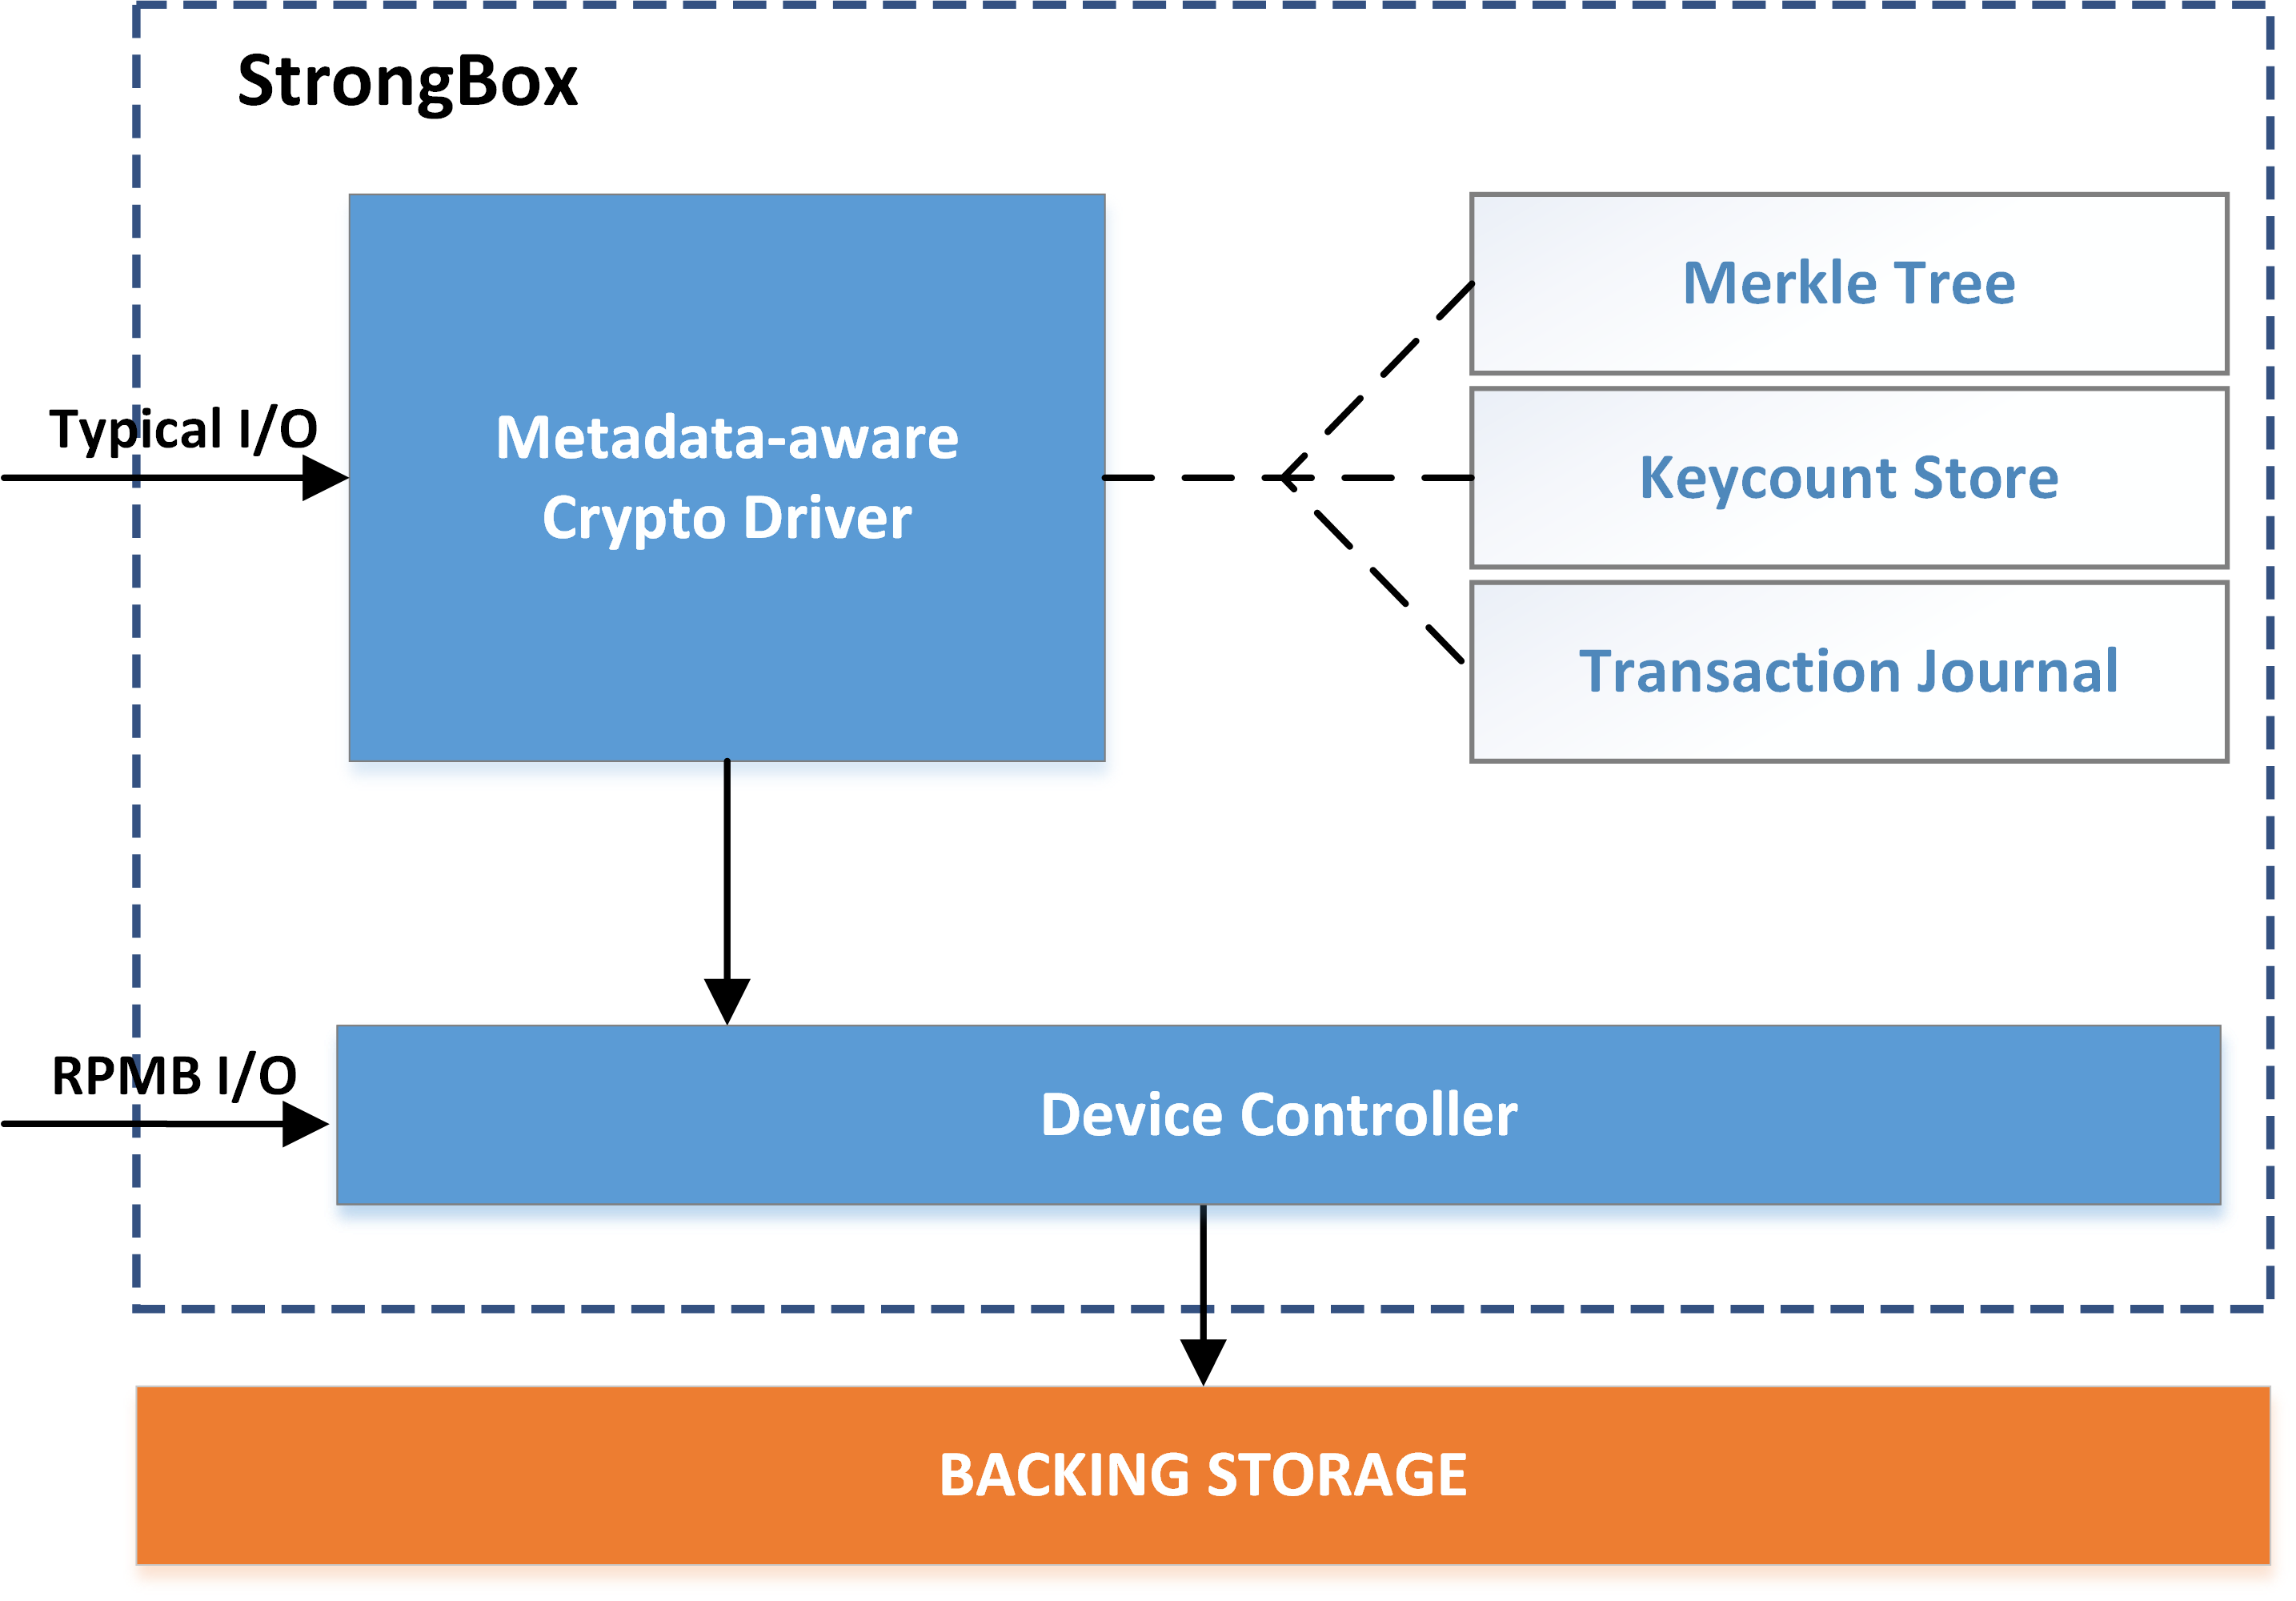
\includegraphics[width=\linewidth]{overview.png}
    \caption{Overview of the SwitchBox construction.}\label{fig:overview}
  \end{figure}

SwitchBox, like StrongBox and Adiantum, is a translation layer positioned
between the block layer and the operating system's virtual file
system~\cite{StrongBox}. There are several places SwitchBox could be implemented
in the system stack: as part of an actual kernel Log-structured File System
(LFS) module like the F2FS filesystem, as a block device or virtual block device
in the manner of dm-crypt, or within a device controller such as an SSD drive
controller's FTL~\cite{StrongBox}.

\figref{overview} illustrates the SwitchBox design. SwitchBox manages five
metadata components: an in-memory \emph{Merkle Tree}; two drive-backed byte
arrays, \ie{the \emph{Keycount Store} and the \emph{Transaction Journal}}; a
globally persistent cryptographically secure monotonic counter; and a flexible
drive-backed store for per-nugget cipher-specific metadata. For our monotonic
counter implementation, we used a \emph{Replay Protected Memory Block} (RPMB).
\TODO{Citation would be good here. But, it is a little strange to get so
specific in this part of the text. I would either save it for a later
implementation section (or evaluation). Or, if you think that the existence of
these counters might be controversial, then say we use RPMB, but we could have
used many others such as...}

These five components are tightly integrated into the cryptographic driver,
which handles data encryption, decryption, overwrite detection, integrity
protection, communication with the wider system to determine the active cipher,
and the application of cipher switching strategies. The cryptographic driver
interacts with 1) the overlying LFS through traditional I/O passed through the
Linux Virtual Filesystem Switch (VFS) as well as 2) the underlying backing store
through the device controller block I/O layer.

SwitchBox uses IPC to receive commands to toggle the active cipher between the
primary and secondary ciphers. \TODO{Spell out the acronym the first time it is
used.}

\begin{figure}[t]
 \centering
 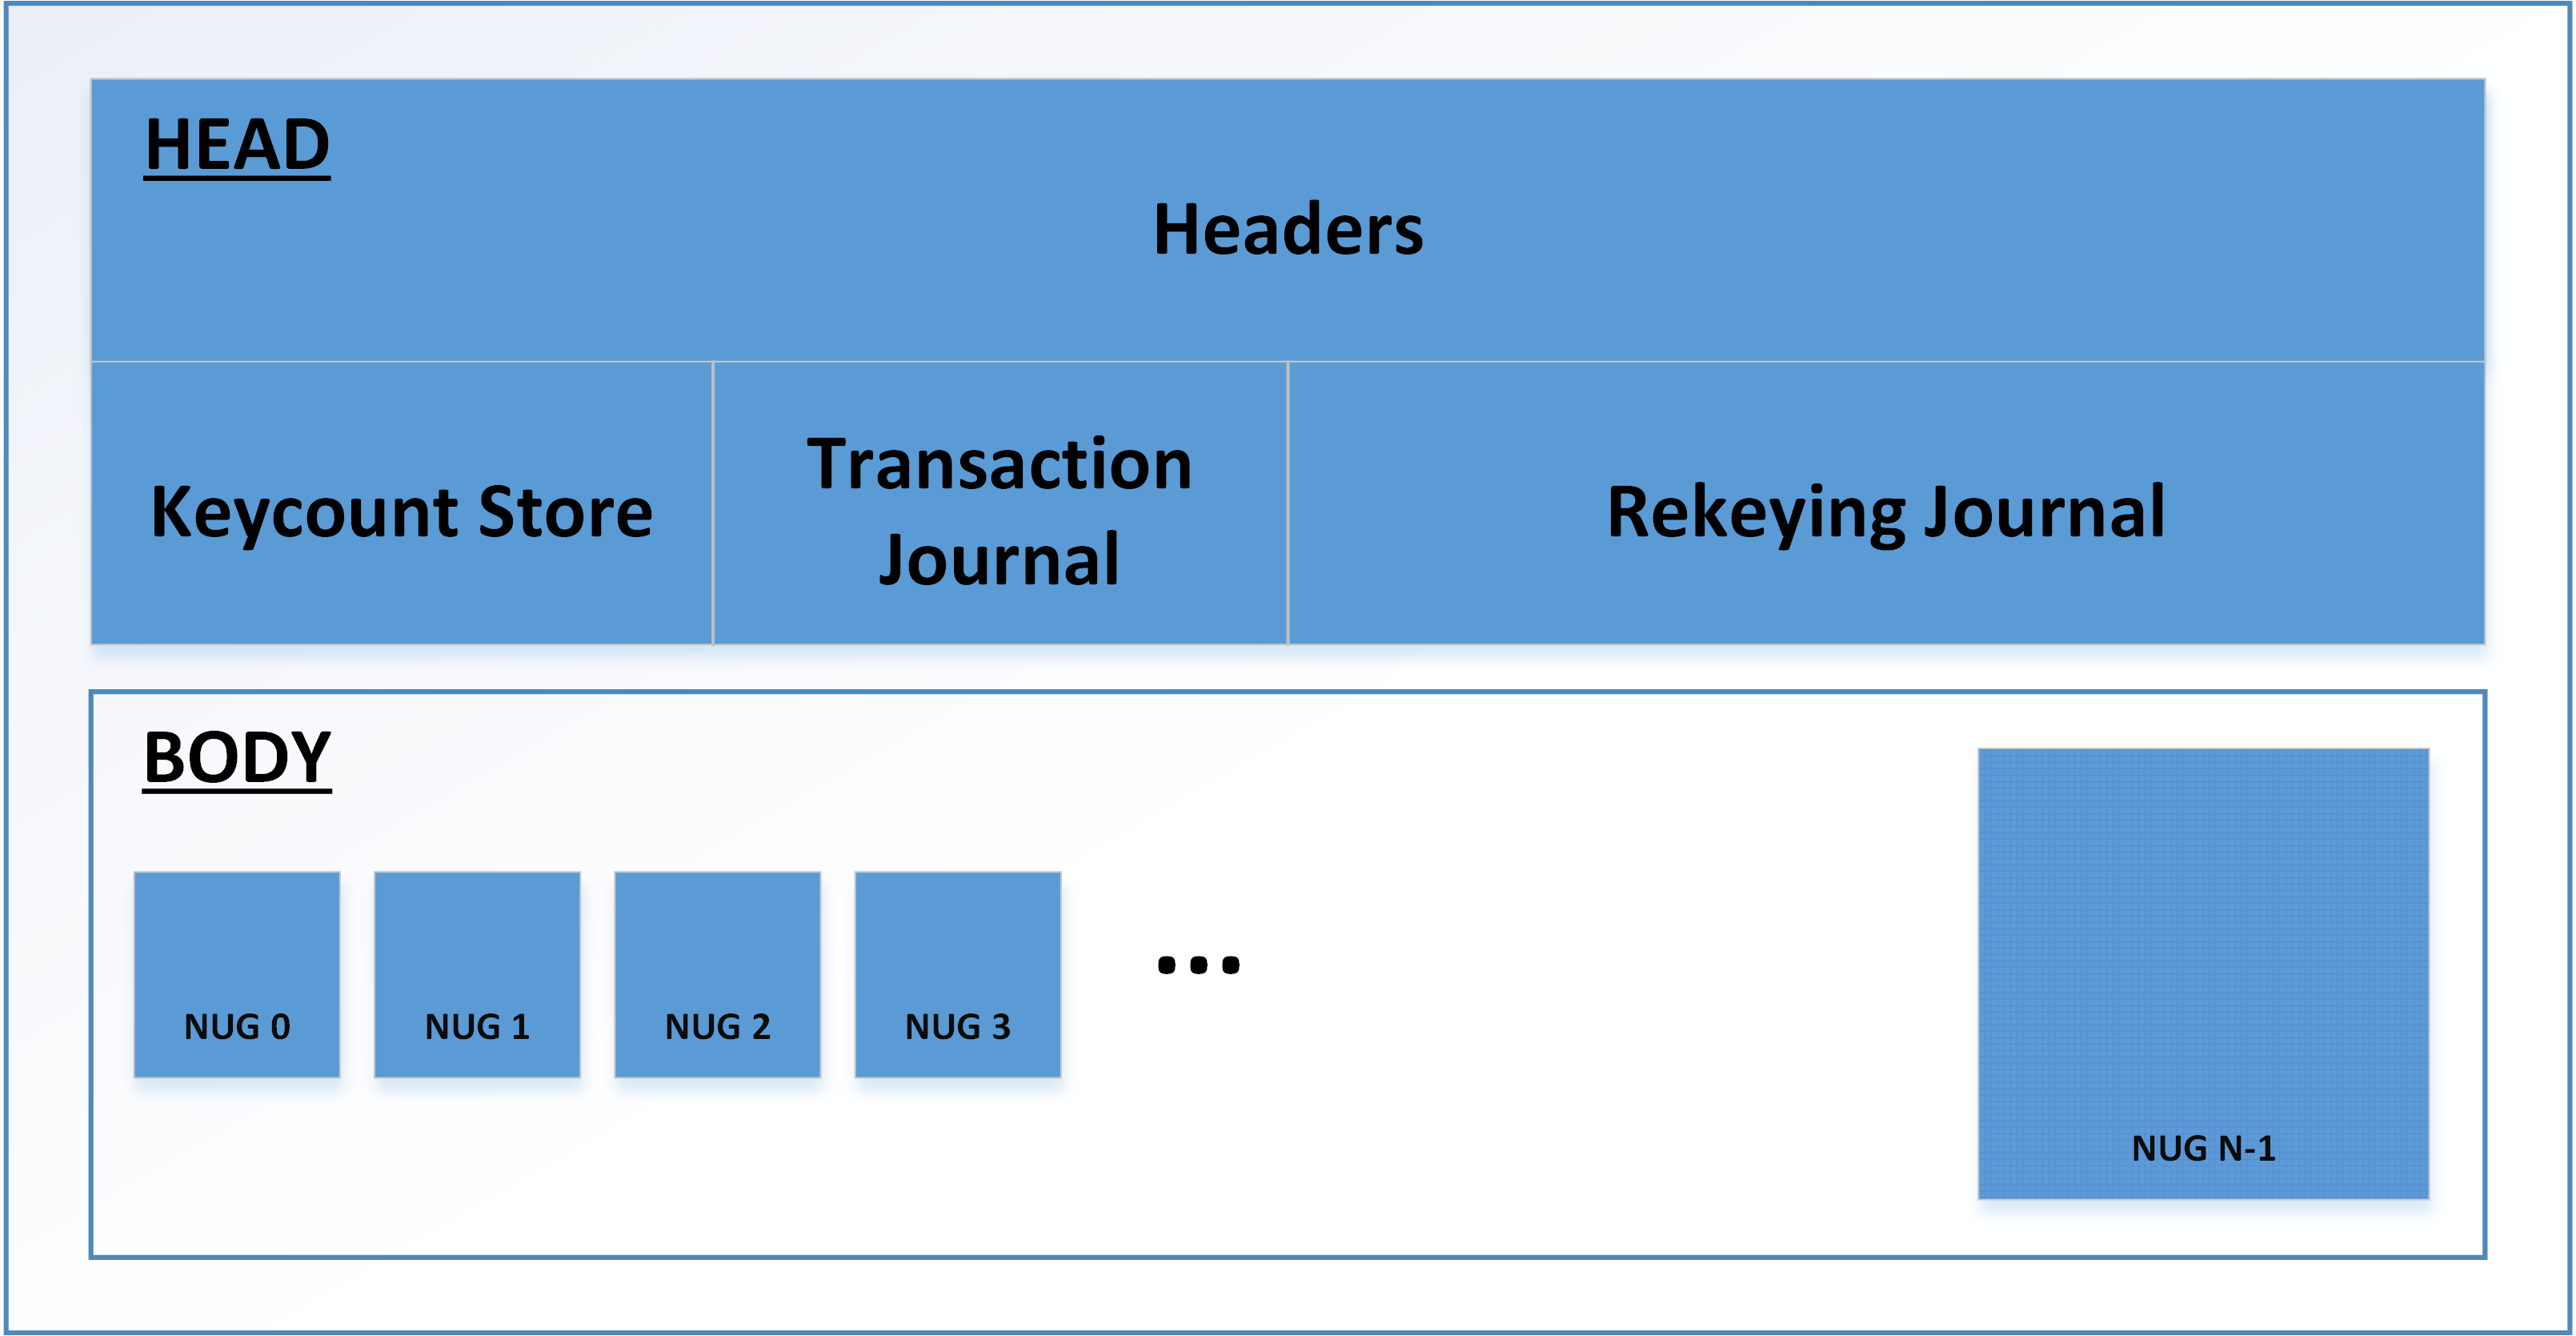
\includegraphics[width=\linewidth]{backstore.png}
  \caption{Layout of SwitchBox's backing storage.}\label{fig:backstore2}
\end{figure}

The backing store is the storage medium SwitchBox operates on. The layout of the
backing store is illustrated in \figref{backstore2}. In the \textit{body} section
of the backing store layout, end-user data is partitioned into a series of
same-size \emph{logical blocks}---which are distinct from the concept of
\emph{physical drive blocks}---we refer to these wider logical blocks as
\emph{nuggets}, marked \textit{NUG}. Hence, a nugget consists of one or more
physical drive blocks along with per-nugget metadata indicating if the nugget
was encrypted with the primary or the secondary cipher. \TODO{Do we redescribe
the rest of the backing store from StrongBox, or should we link to the original
paper? Or should we skip talking about the backing store at all and more briefly
describe nuggets here? It's all not very different from StrongBox's, i.e. an
extra header was added.}

In the rest of this section, we describe our cipher switching strategies. We
also discuss the pluggable stream cipher API and other design challenges. This
is followed by an explanation of implementation-specific details and a
discussion of the overall implications and limitations of SwitchBox's design.

\subsection{Cipher Switching Strategies}

Upon initialization, prior work requires a single cipher to be selected. The
specified cipher---ideally along the pareto frontier of security and energy
tradeoffs---is then used to encrypt and decrypt all data on the filesystem. With
SwitchBox, however, \emph{a pair of ciphers are selected} upon initialization,
depending on the concerns of the end-user. These ciphers are referred to as the
\emph{primary cipher} and the \emph{secondary cipher} respectively, and
represent the static configuration points along the pareto frontier between
which SwitchBox can navigate. \TODO{Do you really have to know these ahead of
time? If I had a cipher API and managed the implementation as a DLL, could I
switch to any cipher, by just building a new DLL? Is there any reason, you
couldn't have three or four or N ciphers and switch between all of them? I ask
all these questions because I want you to separate the conceptual idea, which
should be as broad as possible, from the specific choices you had to make to
demonstrate the idea (which may be much more restricted). Here we want to
discuss the conceptual ideas and save details for the implementation.}

At any moment, the currently active cipher is used to interact with the backing
store. Initially, the primary cipher is the active cipher. Until the wider
system indicates that SwitchBox should use a different cipher to interact with
the backing store, SwitchBox functions identically to StrongBox in that it uses
the primary cipher to encrypt and decrypt all nuggets during I/O.

However, switching the active cipher dynamically allows SwitchBox to achieve
optimal configuration points that are otherwise unachievable with prior work.
The wider system determines if the primary or secondary cipher should be the
active cipher at any given moment, and SwitchBox responds immediately.
Unfortunately, it is entirely non-trivial to determine \emph{when} to re-encrypt
a nugget with a different cipher and \emph{where} to direct the output of that
cipher. \TODO{Don't just say it is difficult, make an argument about why it is
difficult. It is often very helpful to say things that are obvious to you
because they won't be obvious to the reader, but will help build intuition for
what is coming. For example, you can say that one simple approach would
immediately convert the entire drive, but the cost of doing that conversion
might consume more energy than would be saved in future accesses. I do like
using where and when to set up spatial and temporal switching. }

Hence, cipher switching \emph{strategies} are the mechanism by which SwitchBox
can effectively transition nuggets between different encrypted states
dynamically, thus providing a mechanism to navigate the tradeoff space presented
in \figref{40mb-read-with-forward}. \TODO{Expound on this all more? Reword?
Delete? Different chart referenced here instead?} \TODO{Hank: expound! Go ahead
and say that when to target the new encryption is temporal switching and we
propose a specific strategy, \emph{Forward}, to handle it. Where to switch is
spatial switching and we propose two strategies to deal with that.}

\subsubsection{Forward Switching Strategy}

SwitchBox allows each individual nugget to exist encrypted using one cipher or
the other regardless of the currently active cipher. When a nugget is
encountered during I/O that is encrypted using a cipher other than the active
cipher, however, the forward strategy dictates that this nugget be re-encrypted
"just-in-time" using the active cipher before completing the I/O operation. If a
particular nugget encrypted with the non-active cipher is never encountered
during I/O, it is never re-encrypted and remains on the backing store in its
original state. In this way, the forward strategy represents a form of temporal
cipher switching.

Rather than re-encrypt the entire backing store every time the active cipher
changes, this strategy limits the performance impact of cipher switching to
individual nuggets. Similar to rekeying in the original StrongBox construction,
the heavy price of re-encryption is paid only once during the initial
re-encryption, after which the nugget is accessed normally during I/O until the
active cipher is switched again.

There are several forms the forward strategy can take. The default and most
intuitive is \emph{0-forward}, in which SwitchBox immediately transitions
individual nuggets encountered during I/O to the active cipher is they are not
using it. Over time, if various I/O operations end up touching every nugget in
the backing store, the encrypted state of every nugget will eventually become
consistent with the currently active cipher.

The forward strategy can also take the form of \emph{N-forward}, where SwitchBox
attempts to take advantage of spatial sequential locality to transition whole
sets of nuggets into the active cipher. We can trivially expand the forward
strategy to encompass the entire backing store by selecting N equal to the total
number of nuggets managed by SwitchBox. This would have the overhead of
re-encrypting large swaths of the backing store upon every I/O operation where a
nugget encrypted with the non-active cipher is encountered. Of course, this has
the same effect as simply re-initializing the entire filesystem with the new
cipher.

\subsubsection{Selective Switching Strategy}

When SwitchBox is initialized with the selective strategy, the backing store is
partitioned into two regions governed exclusively by the primary and secondary
ciphers, respectively. All nuggets in the first partition are encrypted with the
primary cipher while all nuggets in the second partition are encrypted with the
secondary cipher.

Hence, unlike the forward strategy, which schedules individual nuggets to be
re-encrypted at some point in time \emph{after} the active cipher is switched,
the selective strategy allows the wider system to indicate \emph{where} on the
backing store a read or write operation should occur: either in one partition or
the other. In this way, the selective strategy represents a form of spatial
cipher switching where different regions of the backing store can store
different pieces of data.

\subsubsection{Mirrored Switching Strategy}

Similar to the selective strategy, when SwitchBox is initialized with the
mirrored strategy, the backing store is partitioned into two regions governed
exclusively by the primary and secondary ciphers, respectively. All nuggets in
the first partition are encrypted with the primary cipher while all nuggets in
the second partition are encrypted with the secondary cipher.

However, unlike the selective strategy, all write operations that hit one
partition are mirrored into the other partition immediately. The mirrored
strategy allows the wider system to indicate where on the backing store a
\emph{read} operation should occur. As a result, both regions of the backing
store will always be in a consistent state and share the same data. In this way,
the mirrored strategy, like the selective strategy, represents a form of spatial
cipher switching.

\subsection{Pluggable Stream Cipher API}

\TODO{Always use present tense in technical writing. It should be we develop
instead of we developed.} We developed an API to allow any stream cipher or any
cipher that can pose as a stream cipher to be used with SwitchBox without
modification, including ciphers with residual output, \eg{Freestyle}. \TODO{I
don't know what residual output is, so please expand on the differences between
ciphers that causes problems. But before you do, see the note below on
challenges.} SwitchBox exposes a common encryption and decryption interface,
including read and write handles, that allow SwitchBox to transition nuggets
between arbitrary ciphers at the behest of the wider system. \TODO{This section
is odd here. Having a whole subsection seems to imply that it is as important
as the switching strategies, but having a short paragraph implies it is more of
a side note. In addition, it is not clear what purpose this discussion serves.
I think you need more setup about how different stream ciphers might appear to
all be interchangeable, but they are not, so we need a common interface---again,
sometimes it is actually helpful to state what feels obvious to you.}

\subsection{Additional Challenge: Beware Naive Forward Switching}

It is tempting to implement forward switching such that a nugget is re-encrypted
during I/O if its metadata indicates that it was previously encrypted using the
non-active cipher. However, such a naive implementation can have disastrous
effects on performance depending on the workload.

First, a nugget is considered "pristine" if it has not had any data written into
it yet. SwitchBox determines if a nugget is pristine by checking the state of
the transaction journal for that nugget. A pristine nugget will have a clean
transaction journal.

All nuggets start out as pristine. All nuggets start out with metadata
indicating that they're to be encrypted and decrypted by the primary cipher
(which is the initially active cipher when SwitchBox is first initialized). This
is true \emph{even if the nugget has not been written to yet}. This means, on
read and write operations after the secondary cipher becomes the active cipher
using a naively implemented forward switching strategy, every write operation
will trigger a re-keying, which carries significant overhead.

The solution is to divide forward switching into \emph{soft re-encryption} and
\emph{hard re-encryption}. Fortunately, the SwitchBox design lends itself nicely
to such a distinction for free, as per-nugget metadata is managed separately
from a nugget's actual data.

During soft re-encryption, only the nugget's metadata is changed to indicate
that the nugget can be encrypted and decrypted with the newly active cipher but
\emph{without actually re-encrypting the nugget data itself}. This keeps the
nugget in a "pristine" condition, preserving SwitchBox's ability to write data
into it without triggering a costly rekeying operation every time, preserving
the original StrongBox's performance advantage. At the same time, SwitchBox can
now use the newly active cipher to interact with the nugget as expected.

On the other hand, during hard re-encryption, the nugget's metadata is changed
to match the active cipher \emph{and} the nugget data is re-encrypted using the
new cipher. When using forward switching other that 0-forward, \ie{N-forward}
where $N > 0$, only read operations are allowed to trigger hard re-encryption
for nuggets other than the currently active nugget. This is still not enough to
preserve StrongBox's performance advantage, however, as I/O operations can span
multiple nuggets, and attempting to take advantage of spatial locality after
interacting with every nugget is counterproductive. Hence, only the last nugget
touched by a read or write operation will trigger the more aggressive N-forward
behavior if $N > 0$.

These considerations have the effect of 1) preserving the original StrongBox
performance advantage over prior work and 2) allowing more aggressive N-forward
behavior (where $N > 0$) to take advantage of spatial locality during read-heavy
workloads to result in a further performance advantage (c.f.
\secref{evaluation}).

\subsection{Threat Models}

\TODO{Hank: I feel like we need some discussion of threat model or something.
For example, I really like the mirroring strategy, but I think it breaks if an
attacker has physical access to the drive, right? Like if they have to request
IO through the OS, I think it works becuase the os or hypervisor can hide the
mirrored side, but you can't hide that if I can just read bytes off the drive
itself, right? Sort of similar for forward. We really do need to say something
about when these are applicable and when they aren't.}

\section{Implementation}

\TODO{Mention StrongBox much less, ideally not at all}

Our SwitchBox implementation consists of 9,491 lines of C code; our test suite
consists of 6,077 lines of C code. All together, our solution is comprised of
15,568 lines of C code.

SwitchBox uses OpenSSL version 1.1.0h and LibSodium version 1.0.12 for its
AES-XTS and AES-CTR implementations. Open source ARM NEON optimized
implementations of ChaCha are provided by Floodyberry~\cite{Floodyberry}. The
Freestyle cipher reference implementation is from the original Freestyle
paper~\cite{Freestyle}. The eSTREAM Profile 1 cipher implementations are from
the open source libestream cryptographic library~\cite{libestream} by Lucas
Clemente Vella. As with the original StrongBox construction, the Merkle Tree
implementation is from the Secure Block Device~\cite{SBD}. SwitchBox
implementation is publicly available open-source\footnote{\SystemURI}.

For a fair comparison with the original StrongBox implementation, we mirror
their use of the BUSE~\cite{BUSE} virtual block device as our device controller.
BUSE is a thin (200 LoC) wrapper around the standard Linux Network Block Device
(NBD). BUSE allows an operating system to transact block I/O requests to and
from virtual block devices exposed via domain socket.

For the purposes of our implementation, we make the choice of ciphers binary:
either the system wants SwitchBox to access the backing store using the primary
cipher or the secondary cipher. However, there is no technical limitation
preventing various different nuggets encrypted with three, four, or more unique
ciphers from co-existing on the backing store. \TODO{Good detail. In this case,
remove the discussion above about how we just support two ciphers.}

\subsection{Indicating a Cipher Switch Should Occur}

When SwitchBox should be using the primary cipher or the secondary cipher to
interact with the backing store, this intent is communicated via POSIX message
queue in our implementation. It is not a requirement of SwitchBox that a POSIX
message queue be used over any other method of inter-process communication (IPC)
so long as SwitchBox is notified asynchronously when the wider system desires
one cipher be active over the other. \TODO{I am not sure why this section is
here. It is either too much detail, or more likely there is some important
issue, but whatever that is needs to be stated much more explicitly. Like maybe
the problem is that the use needs to actually communicate with the SwitchBox
implementation and we need a mechanism to do that? Anyway, assuming you expand
this a little so it is clear what problem is being addressed, then you can just
make this another paragraph in implementation instead of splitting it out into a
subsub.}

\TODO{I think the discussion here only covers temporal switching. I believe you
should indicate that for this paragraph and then have a second paragraph that
talks about how to indicate that a spatial switch should occur (and you might
need a different method for mirrored and selective). Correct me if I am wrong,
but I believe that the selective switch will require the IOp to indicate that
this data needs to be handled in one way or another.}

\subsection{Backing Store Initialization}

To operate securely, SwitchBox must be seeded with random data initially rather
than have the backing store consist of all zeroes. This is a one-time cost paid
during initialization and has no tangible effect on performance.

If nuggets are not seeded with random data initially, any write operation into
an "empty" nugget might leak information or constitute an overwrite where the
predictable state of the backing store (\ie{initialized to all zeroes}) leads to
an overwrite-style condition.

\section{Evaluation}\label{sec:evaluation}

\subsection{Experimental Setup}

We implement SwitchBox on a Hardkernel Odroid XU3 ARM big.LITTLE system with
Samsung Exynos 5422 A15/A7 heterogeneous multi-processing quad core CPUs at
maximum clock speed, 2 gigabyte LPDDR3 RAM at 933 MHz, and an eMMC5.0 HS400
backing store running Ubuntu Trusty 14.04.6 LTS, kernel version 3.10.106.

We evaluate SwitchBox using a RAM disk. The maximum theoretical memory bandwidth
for this Odroid model is 14.9GB/s\@. Our observed maximum memory bandwidth is
4.5GB/s.

We evaluate SwitchBox on two high level workloads: sequential and random I/O. In
both workloads, a number of bytes are written and then read (either 4KB, 512KB,
5MB, 40MB) 10 times. This experiment is repeated three times. When evaluating
switching strategies, a finer breakdown in workloads is made using a
pre-selected pair of ciphers, yielding a ``cipher configuration'' point given a
switching strategy: a specific ratio of those 10 write-read pairs is performed
using one cipher and the remainder with the other. There are three ratios we use
to evaluate SwitchBox's performance: 1:3, 1:1, and 3:1. Respectively, that's 1
whole file write-read operation in the secondary cipher for every 3 whole file
write-read operations in the primary cipher (1:3), 1 whole file write-read
operation in the secondary cipher for every other whole file write-read
operation in the primary cipher (1:1), and 3 whole file write-read operations in
the secondary cipher for every 1 whole file write-read operation in the primary
cipher (3:1).

In this section we answer the following questions:
\begin{enumerate}
 \item Can SwitchBox reach security/energy tradeoffs that are not reachable with prior work?
 \item What switching strategy works best in which scenario?
 \item What is the performance overhead of each cipher switching strategy?
 \item What is the storage overhead of each cipher switching strategy?
 \item How does incorporation of cipher-switching change the threat analysis?
\end{enumerate}

\subsection{Reaching Between Static Configuration Points}

\begin{figure*}[ht] \textbf{Baseline Cipher I/O Performance}\par\medskip
  \centering
  {\input{charts/tradeoff-no-ratios.tex}} \caption{Median sequential and random
  read and write latency per I/O operation size (4KB, 512KB, 5MB, 40MB) using
  multiple cipher configurations achievable without switching and ordered by
  security score.}
 \label{fig:tradeoff-no-ratios}
\end{figure*}

\figref{tradeoff-no-ratios} shows the security score versus I/O latency tradeoff
between our different stream ciphers when completing a 40MB read of encrypted
storage. The experiment was performed on a Linux RAM disk on an ARM big.LITTLE
Exynos Octa processor, which is similar to the processors used in the Samsung
Galaxy line of phones and other devices. Of the ciphers we tested, those with
more desirable but performance inhibitive security properties (see:
\secref{design}) resulted in higher latency for I/O operations while ciphers
with relatively weaker less desirable security properties resulted in lower
latency.

\begin{figure*}[ht]
  \textbf{Forward Switching I/O Ratio Performance}\par\medskip
  \centering
  {\input{charts/tradeoff-with-ratios.tex}} \caption{Median sequential and
  random read and write latency per I/O operation size (4KB, 512KB, 5MB, 40MB)
  using multiple cipher configurations ordered by security score. With Forward
  switching, we achieve additional configurations unachievable with prior work
  incapable of switching.}
 \label{fig:tradeoff-with-ratios}
\end{figure*}

\TODO{Add discussion of the different sizes and how they relate. Add exhaustive
set of charts and then something that says these trends are similar across
workloads, so from now on we just focus on 5MB}

\subsection{Switching Strategies Under Various Workloads}

\TODO{There should be a description of exactly how the experiments were setup to
answer this question, a description of the chart (what are the axes, what are
the points/lines/bars), a textual description of the results in the chart, and
then the conclusion we can draw regarding the question for that subsection.}

\subsection{Cipher Switching Overhead}

\TODO{There should be a description of exactly how the experiments were setup to
answer this question, a description of the chart (what are the axes, what are
the points/lines/bars), a textual description of the results in the chart, and
then the conclusion we can draw regarding the question for that subsection.}

\subsection{Augmented Threat Analysis}

\TODO{Reuse the table from the strongbox paper, but have a different column for
forward, selective, and mirrored.}



\TODO{Move all the following analysis into their proper subsections above.}

\figref{tradeoff-with-ratios} shows the 40MB read performance of three ciphers:
ChaCha8, ChaCha20, and Freestyle in its ``fast'' configuration. This illustrates
the tradeoff space between latency/energy and security for these three static
discrete pareto optimal configurations achievable offline via prior work.

\figref{tradeoff-with-ratios} additionally illustrates the flexibility of
SwitchBox using the 0-forward switching strategy to reach pareto optimal dynamic
configuration points \emph{between} traditional static configuration in the
tradeoff space that are unachievable via prior work.

\begin{figure*}[ht]
   \textbf{Mirrored and Selective Switching I/O Ratio Performance}\par\medskip
   \centering
   {\input{charts/mirrored-selective-baseline.tex}} \caption{Median sequential
   and random read and write latency per I/O operation size (4KB, 512KB, 5MB,
   40MB) using multiple cipher configurations ordered by security score;
   performance comparison of Mirrored and Selective switching strategies to
   baseline.}
  \label{fig:mirrored-selective-baseline}
\end{figure*}

\figref{mirrored-selective-baseline} show the the performance of forward,
mirrored, and selective strategies against two 40MB read and write workloads:
Freerun and WORM. \TODO{Explain these two workloads.} Additionally, the time
required to transition the entire backing store from one cipher to the other is
included \TODO{This is ``time to cipher switch'' or TTCS, but this is renamed in
the actual figure.}

1-forward and 2-forward have overhead that makes them slower than forward 0 for
sequential and random freerun. However, WORM workload shows 1-forward
outperforming 0-forward by \TODO{include percentage (it's small)}. This is
because WORM workload characteristics allow benefits of more aggressive forward
switching to be realized \TODO{Elaborate more here}.

The mirrored and selective switching strategies achieve read parity with the
static cipher configurations, hence their performance. However, mirrored stacks
write latency of both ciphers in the pair because writes are mirrored across
both partitions. On the other hand, selective switching achieves write parity
with the static configuration. Mirrored and selective are not preferable to
forward in all circumstances because drive space is traded off; in our
experiments, half the drive is lost to partitioning.

\TODO{Word these paragraphs better. Include numbers from chart to be more
specific.}

Selective is usually preferable to mirrored due to Mirrored strategy's egregious
write overhead. However, forward and selective take a comparatively long time to
transition the entire backing store from one cipher to the other while mirrored
can achieve this virtually instantaneously. If it is not desirable to maintain
both encrypted versions of data on the backing store, one partition or the other
can be TRIM-ed and the data deleted relatively quickly. On the other hand, when
using the Selective strategy, it is not possible to transition the backing store
entirely to one cipher or another (hence no bar for TTCS). For the forward
strategy, it takes a long time. \TODO{Specific numbers from chart need to go in
here.}

\section{\SYSTEM{} Case Studies} \label{sec:usecases}

\TODO{At a high-level, all of these are good, but the devil is always
  in the details. I think it is important to get them as fully
  fleshed-out as possible as soon as possible.  I really want to see
  the real data and see the discussion about what happens if a user
  was forced to reconfigure.  If you already have the data and just
  haven't added the real charts yet, you could also spend some time
  just writing the text that will go with them. }

\subsection{Intra-file Variable Security Regions (VSR)}

Communicating classified materials, grand jury testimony, corporate secrets,
etc. require the highest level of discretion when handled, yet sensitive
information like this often appears within a (much) larger amount of data that
we care less about in context.

In this scenario, a user wants to indicate one or more regions of a file are
more sensitive than the others. For example, perhaps banking transaction
information is littered throughout a document; perhaps passwords and other
sensitive or compromising information exists within a much larger data file.
This sensitive information would be encrypted using a less performant (sometimes
dramatically so) cipher in exchange for a stronger security guarantee.

The user will not experience a significant performance hit when perusing the
data if the bulk of it is encrypted using a high performance cipher.
Simultaneously, the more sensitive data regions are future-proofed and more
resilient to attack using a high security cipher.

A "VSR" is a region of a file that is crypted with the alternative
rather than the primary cipher that encrypts the remaining majority of the file.

Benefit: we can "future-proof" our encrypted highly sensitive data against more
powerful future attacks/less trustworthy ciphers while preserving the
performance win from using a faster less secure cipher.

\begin{figure}[ht]
 \centering
  \includegraphics[width=\linewidth]{drawn/8.png}
   \caption{\TODO{Caption goes here}}\label{fig:mirrored-vs-selective}
\end{figure}

\subsection{Balancing Security Goals with a Constrained Energy Budget}

When our mobile devices enter power saving mode, it is usually because the total
energy/power budget for the device has become constrained for one reason or
another.

When a device enters this mode, all software and components are configured by
the OS to use as little of the available energy as possible. The filesystem
should be made to behave in a manner that is energy-aware as well.

Our goal is to use as little energy as possible (while reasonably preserving
filesystem performance) until the energy budget changes or the device dies.

Benefit: When constantly streaming data, e.g. using DLNA to stream a high
resolution video wirelessly to a TV on the same network, the ability to adapt to
time-varying data rates and QoS requirements while maintaining confidentiality
and integrity guarantees is paramount. This can be done by trading off a set of
security guarantees with respect to the energy spent crypting each bit. With
cipher switching, the filesystem can react dynamically to the system's total
energy budget while still aiming for the most performant (least latency)
configuration.
\TODO{See my earlier comment (in email or some other TODO) about reading vs. writing.  It seems fairly clear to me that you can make this work for writes, but I don't see hwo this works for reads. If the video is stored in a strong cipher, don't you have to decrypt it at that strength?  Where does the energy win come from on reads?}

\begin{figure}[ht]
 \centering
  \includegraphics[width=\linewidth]{drawn/7.png}
   \caption{\TODO{Caption goes here}}\label{fig:energy-budget}
\end{figure}

\subsection{Responding to End-of-Life Slowdown in Solid State Drives}

Due to garbage collection and the append-mostly nature of SSDs and other NAND
devices, as free space becomes constrained, performance drops off a cliff. This
is a well-studied issue (see related work).

If the filesystem is made aware when the backing store is in such a state, we
can offset some of the (drastic) performance loss by swapping the ciphers of hot
nuggets to the fastest cipher available until the disk space problem is
remedied, after which the system can detect return the swapped nuggets to their
former encrypted state.

Benefit: we can mitigate the performance loss of a slowing SSD by using a faster
but less secure cipher.

\begin{figure}[ht]
 \centering
  \includegraphics[width=\linewidth]{drawn/6.png}
   \caption{\TODO{Caption goes here}}\label{fig:eol}
\end{figure}

\subsection{Custody Panic: Securing Device Data Under Duress}

Nation-state and other adversaries have truly extensive compute resources at
their disposal, as well as knowledge of side-channels and access to technology
like q-bit computers.

Suppose one were attempting to re-enter a country through a border checkpoint
after visiting family when one is stopped. Your mobile device is confiscated and
placed in custody of the State. In such a scenario, it would be useful if the
device could swap itself into a more secure state as quickly as possible.

Benefit: greater security guarantee achieved using the highest security
encryption available versus powerful adversaries with unknown means and motive.

\TODO{Dumb question: this scenario assumes you are worried about the data, but can't wipe the drive, right?  Is that a plausible scenario? }
\section{Related Work}\label{sec:related}

The standard approach to FDE, using AES-XTS, introduces significant overhead.
Recently, it has been established that encryption using \emph{stream ciphers}
for FDE is faster than using AES~\cite{StrongBox, AnotherPaper1, AnotherPaper2}.
However, when used naively in drive encryption, stream ciphers are widely known
to be vulnerable to ``overwrite attacks'' like pad reuse and
rollback~\cite{KatzLindell, StrongBox}. To enable FDE using stream ciphers,
prior work explores several approaches:

\begin{itemize}
   \item Use a non-deterministic CTR mode with specially designed cipher and
   filesystem (Freestyle~\cite{Freestyle}).
   \item Use a length-preserving ``tweakable super-pseudorandom permutation''
   construction with nonce-accepting stream cipher (Adiantum~\cite{Adiantum}).
   \item Use a stream cipher in a binary additive (XOR) mode leveraging metadata
   management and Log-structured File Systems' (LFS) overwrite-averse behavior
   to prevent overwrites (StrongBox~\cite{StrongBox}).
\end{itemize}

Unlike StrongBox and other work, which focuses on optimizing performance despite
re-ciphering due to overwrites, SwitchCrypt maintains overwrite protections
while abstracting the idea of re-encrypting nuggets out into cipher switching;
instead of myopically pursuing a performance win, this allows the trade off of
various cipher configurations dynamically.

However, trading off security for energy, performance, and other concerns is not
a new idea~\cite{ScalableSecurity, WolterReinecke, ZengChow1, ZengChow2,
HaleemEtAl, LiOmiecinski}. For instance, Goodman et al. (1998) introduced
trading decreased security for saving energy dissipated to encrypt a bit during
wireless communication~\cite{ScalableSecurity}. Similar in intent to VSRs,
Goodman minimizes energy consumption by separating low-priority communications
from high-priority and encrypting them differently. Goodman et al.'s approach is
designed for communication and only considered changing key lengths, thus it did
not anticipate the need for SwitchCrypt's generic API, switching strategies, or
security scores. Further, Wolter and Reinecke study performance and security
tradeoffs, exploring approaches to quantifying security in several
contexts~\cite{WolterReinecke}. \TODO{Again, need to say something more to
differentiate us.  Something like: "This study anticipates the value of
dynamically switching ciphers but proposes no mechanisms to actually enable this
switch."}

In the wild, companies like Google~\cite{AndroidM} and Apple~\cite{iOSFDE} have
explored performance-security tradeoffs in hardware when considering FDE
support. Google's Adiantum uses a less secure reduced round version of
ChaCha~\cite{Adiantum}. LastPass (LogMeIn) has dealt with scaling the number of
iterations of its PBKDF\#2, trading performance for security~\cite{LastPass}. \TODO{Need a summary sentence here, too.  Again, need to make it clear that what we are doing is related to this work, but solved many novel challenges.}

\section{Conclusion}\label{sec:conclusion}
%This paper advocates for a more agile approach to full 
%drive encryption where the storage system can dynamically 
%alter the tradeoffs between security and latency (or energy) 
%for data at rest.  To support this vision of agile encryption,
%we have proposed an API that allows mulitple stream ciphers, with 
%different input and output characteristics to be composed in a 
%generic manner.  We have identified three strategies for using 
%this API to switch ciphers dynamically, but with low overhead.  
%We have also proposed a scoring method for determining when to 
%use one cipher over another. Our case studies show how different 
%strategies can be used to achieve different goals in practice.
%We believe that agile encryption will become increasingly important 
%as successful operation of computer systems increasingly requires 
%balancing seemingly conflicting operational requirements.  We hope 
%that this work inspires further research into achieving this balance, 
%including both mechanisms and policies for exposing and navigating 
%the underlying tradeoff spaces. TODO

Stream ciphers are fast and offer strong security properties, but optimizing for
performance often conflicts with other key concerns. In this paper we presented
SwitchCrypt to navigate the security and latency/energy tradeoff space via
\emph{cipher switching} in space and time. We provided empirical results
demonstrating the conditions under which different switching strategies are
optimal and explored four related cases. In all cases, we found that SwitchCrypt
achieves reduced energy usage and I/O latency compared to static approaches.
Perhaps more importantly, though, in all cases SwitchCrypt achieves flexibility
that is simply not possible with prior designs.  We hope that this work inspires
further research into balancing competing security, energy, and performance
tradeoffs, including both mechanisms and policies for exposing and navigating
these tradeoff spaces.

\PUNT{\TO\DO{Add David to acknowledgements once we get out of anon reviews.}}

\input{9_acks}

% Uncomment to show all citable references:
% \cite{*}

%% Start a new page for your references:
\clearpage

%% Test printing all refs:
%\nocite{*}

%% If using natbib:
\bibliographystyle{ACM-Reference-Format}
%\balance % it does not seem to work with this outdated natbib thing
\bibliography{refs}

%% If using biblatex:
%\bibliographystyle{ACM-Reference-Format}
%\balance
%\printbibliography

\end{document}
